\title{Coalescent approaches to phylogeography and Approximate
  Bayesian computation}

A few years before Knowles~\cite{Knowles-2001} appeared Beerli and
Felsenstein~\cite{Beerli-Felsenstein-1999,Beerli-Felsenstein-2001}
proposed a coalescent-based method to estimate migration rates among
populations. As with other analytical methods we've encountered in
this course, the details can get pretty hairy, but the basic idea is
(relatively) simple.\index{coalescent!migration}

Recall that in a single population we can describe the coalescent
history of a sample without too much difficulty. Specifically, given a
sample of $n$ alleles in a diploid population with effective size
$N_e$, the probability that the first coalescent event took place $t$
generations ago is
\begin{equation}
P(t|n, N_e) = \left(\frac{n(n-1)}{4N_e}\right)\left(1-
  \frac{n(n-1)}{4N_e}\right)^{t-1} \quad . \label{eq:coalescent-single}
\end{equation}
Now suppose that we have a sample of alleles from $K$ different
populations. To keep things (relatively) simple, we'll imagine that we
have a sample of $n$ alleles from every one of these populations and
that every population has an effective size of $N_e$. In addition,
we'll imagine that there is migration among populations, but again
we'll keep it really simple. Specifically, we'll assume that the
probability that a given allele in our sample from one population had
its ancestor in a different population in the immediately preceding
generation is $m$.\footnote{In other words, $m$ is the backwards
  migration rate, the probability that a gene in one population came
  from another population in the preceding generation. This is the
  same migration rate we encountered weeks ago when we discussed the
  balance between drift and migration.} Under this simple scenario, we
can again construct the coalescent history of our sample. How? Funny
you should ask.

We start by using the same logic we used to construct
equation~(\ref{eq:coalescent-single}). Specifically, we ask ``What's
the probability of an `event' in the immediately preceding
generation?'' The complication is that there are two kinds of events
possible: (1) a coalescent event and (2) a migration event. As in our
original development of the coalescent process, we'll assume that the
population sizes are large enough that the probability of two
coalescent events in a single time step is so small as to be
negligible. In addition, we'll assume that the number of populations
and the migration rates are small enough that the probability of more
than one event of either type is so small as to be negligible. That
means that all we have to do is to calculate the probability of either
a coalescent event or a migration event and combine them to calculate
the probability of an event. It turns out that it's easiest to
calculate the probability that there {\it isn't\/} an event first and
then to calculate the probability that there is an event as one minus
that.

We already know that the probability of a coalescent event in
population $k$, is
\[
P_k(\mbox{coalescent}|n, N_e) = \frac{n(n-1)}{4N_e} \quad ,
\]
so the probability that there is {\it not\/} a coalescent event in any
of our $K$ populations is
\[
P(\mbox{no coalescent}|n, N_e, K) = \left(1-\frac{n(n-1)}{4N_e}\right)^K
\quad .
\]
If $m$ is the probability that there was a migration event in a
particular population than the probability that there is {\it not\/} a
migration event involving any of our $nK$ alleles\footnote{$K$ populations
each with $n$ alleles} is
\[
P(\mbox{no migration}|m, K) = (1-m)^{nK} \quad .
\]
So the probability that there {\it is\/} an event of some kind is
\[
P(\mbox{event}|n, m, N_e, K) = 1 - P(\mbox{no coalescent}|n, N_e,
K)P(\mbox{no migration}|m, K) \quad .\label{eq:event}
\]
Now we can calculate the time back to the first event
\[
P(\mbox{event at }t|n, m, N_e, K) = P(\mbox{event}|n, m, N_e,
K)\left(1 - P(\mbox{event}|n, m, N_e, K)\right)^{t-1} \quad . \label{eq:time-to-event}
\]
We can then use Bayes theorem to calculate the probability that the
event was a coalescence or a migration and the populations
involved. Once we've done that, we have a new population configuration
and we can start over. We continue until all of the alleles have
coalesced into a single common ancestor, and then we have the complete
coalescent history of our sample.\footnote{This may not seem very
  simple, but just think about how complicated it would be if I
  allowed every population to have a different effective size and if I
  allowed each pair of populations to have different migration rates
  between them.} That's roughly the logic that Beerli and Felsenstein
use to construct coalescent histories for a sample of alleles from a
set of populations{\dash}except that they allow effective population
sizes to differ among populations and they allow migration rates to
differ among all pairs of populations. As if that weren't bad enough,
now things start to get even more complicated.

There are lots of different coalescent histories possible for a sample
consisting of $n$ alleles from each of $K$ different populations, even
when we fix $m$ and $N_e$. Worse yet, given any one coalescent
history, there are a lot of different possible mutational histories
possible. In short, there are a lot of different possible sample
configurations consistent with a given set of migration rates and
effective population size. Nonetheless, some combinations of $m$ and
$N_e$ will make the data more likely than others. In other words, we
can construct a likelihood for our data:
\[
P(\mbox{data}|m, N_e) \propto f(n, m, N_e, K) \quad ,
\]
where $f(n, m, N_e,K)$ is some very complicated function of the
probabilities we derived above. In fact, the function is so
complicated, we can't even write it down. Beerli and Felsenstein,
being very clever people, figured out a way to simulate the
likelihood, and {\tt Migrate} provides a (relatively) simple way that
you can use your data to estimate $m$ and $N_e$ for a set of
populations. In fact, {\tt Migrate} will allow you to estimate
pairwise migration rates among all populations in your sample, and
since it can simulate a likelihood, if you put priors on the
parameters you're interested in, i.e., $m$ and $N_e$, you can get
Bayesian estimates of those parameters rather than maximum likelihood
estimates, including credible intervals around those estimates so that
you have a good sense of how reliable your estimates are.\footnote{If
  you'd like to see a comparision of maximum likelihood and Bayesian
  approaches, Beerli~\cite{Beerli-2006} provides an excellent
  overview.}\index{coalescent!estimating migration rates}\index{migration!estimating}

There's one further complication I need to mention, and it involves a
lie I just told you. {\tt Migrate} can't give you estimates of $m$ and
$N_e$. Remember how every time we've dealt with drift and another
process we always end up with things like $4N_em$, $4N_e\mu$, and the
like. Well, the situation is no different here. What {\tt Migrate} can
actually estimate are the two parameters $4N_em$ and
$\theta=4N_e\mu$.\footnote{Depending on the option you pick when you
  run {\tt Migrate} you can either get $\theta$ and $4N_em$ or
  $\theta$ and $M=m/\mu$.} How did $\mu$ get in here when I only
mentioned it in passing? Well, remember that I said that once the
computer has constructed a coalescent history, it has to apply
mutations to that history. Without mutation, all of the alleles in our
sample would be identical to one another. Mutation is what what
produces the diversity. So what we get from {\tt Migrate} isn't the
fraction of a population that's composed of migrants. Rather, we get
an estimate of how much migration contributes to local population
diversity relative to mutation. That's a pretty interesting estimate
to have, but it may not be everything that we want.

There's a further complication to be aware of. Think about the
simulation process I described. All of the alleles in our sample are
descended from a single common ancestor. That means we are implicitly
assuming that the set of populations we're studying have been around
long enough and have been exchanging migrants with one another long
enough that we've reached a drift-mutation-migration equilibrium. If
we're dealing with a relatively small number of populations in a
geographically limited area, that may not be an unreasonable
assumption, but what if we're dealing with populations of crickets
spread across all of the northern Rocky Mountains? And what if we
haven't sampled all of the populations that
exist?\footnote{Beerli~\cite{Beerli-2004} discusses the impact of
  ``ghost'' populations. He concludes that you have to be careful
  about which populations you sample, but that you don't necessarily
  need to sample every population. Read the paper for the details.} In
many circumstances, it may be more appropriate to imagine that
populations diverged from one another at some time in the not too
distant past, have exchanged genes since their divergence, but haven't
had time to reach a drift-mutation-migration equilibrium. What do we
do then?

\section*{Divergence and migration}

Nielsen and Wakely~\cite{Nielsen-Wakeley-2001} consider the simplest
generalization of Beerli and
Felsenstein~\cite{Beerli-Felsenstein-1999,Beerli-Felsenstein-2001} you
could imagine~(Figure~\ref{fig:nielsen-wakeley}). They consider a
situation in which you have samples from only two populations and
you're interested in determining both how long ago the populations
diverged from one another and how much gene exchange there has been
between the populations since they diverged. As in {\tt Migrate}
mutation and migration rates are confounded with effective population
size, and the relevant parameters become:\index{coalescent!estimating migration}\index{coalescent!diverging populations}

\begin{itemize}

\item $\theta_a$, which is $4N_e\mu$ in the ancestral population.

\item $\theta_1$, which is $4N_e\mu$ in the first population.

\item $\theta_2$, which is $4N_e\mu$ in the second population.

\item $M_1$, which is $2N_em$ in the first population, where $m$ is
  the fraction of the first population composed of migrants from the
  second population.

\item $M_2$, which is $2N_em$ in the second population.

\item $T$, which is the time since the populations
  diverged. Specifically, if there have been $t$ units since
  the two populations diverged, $T=t/2N_1$, where $N_1$ is the
  effective size of the first population.

\end{itemize}

\begin{figure}
\begin{center}
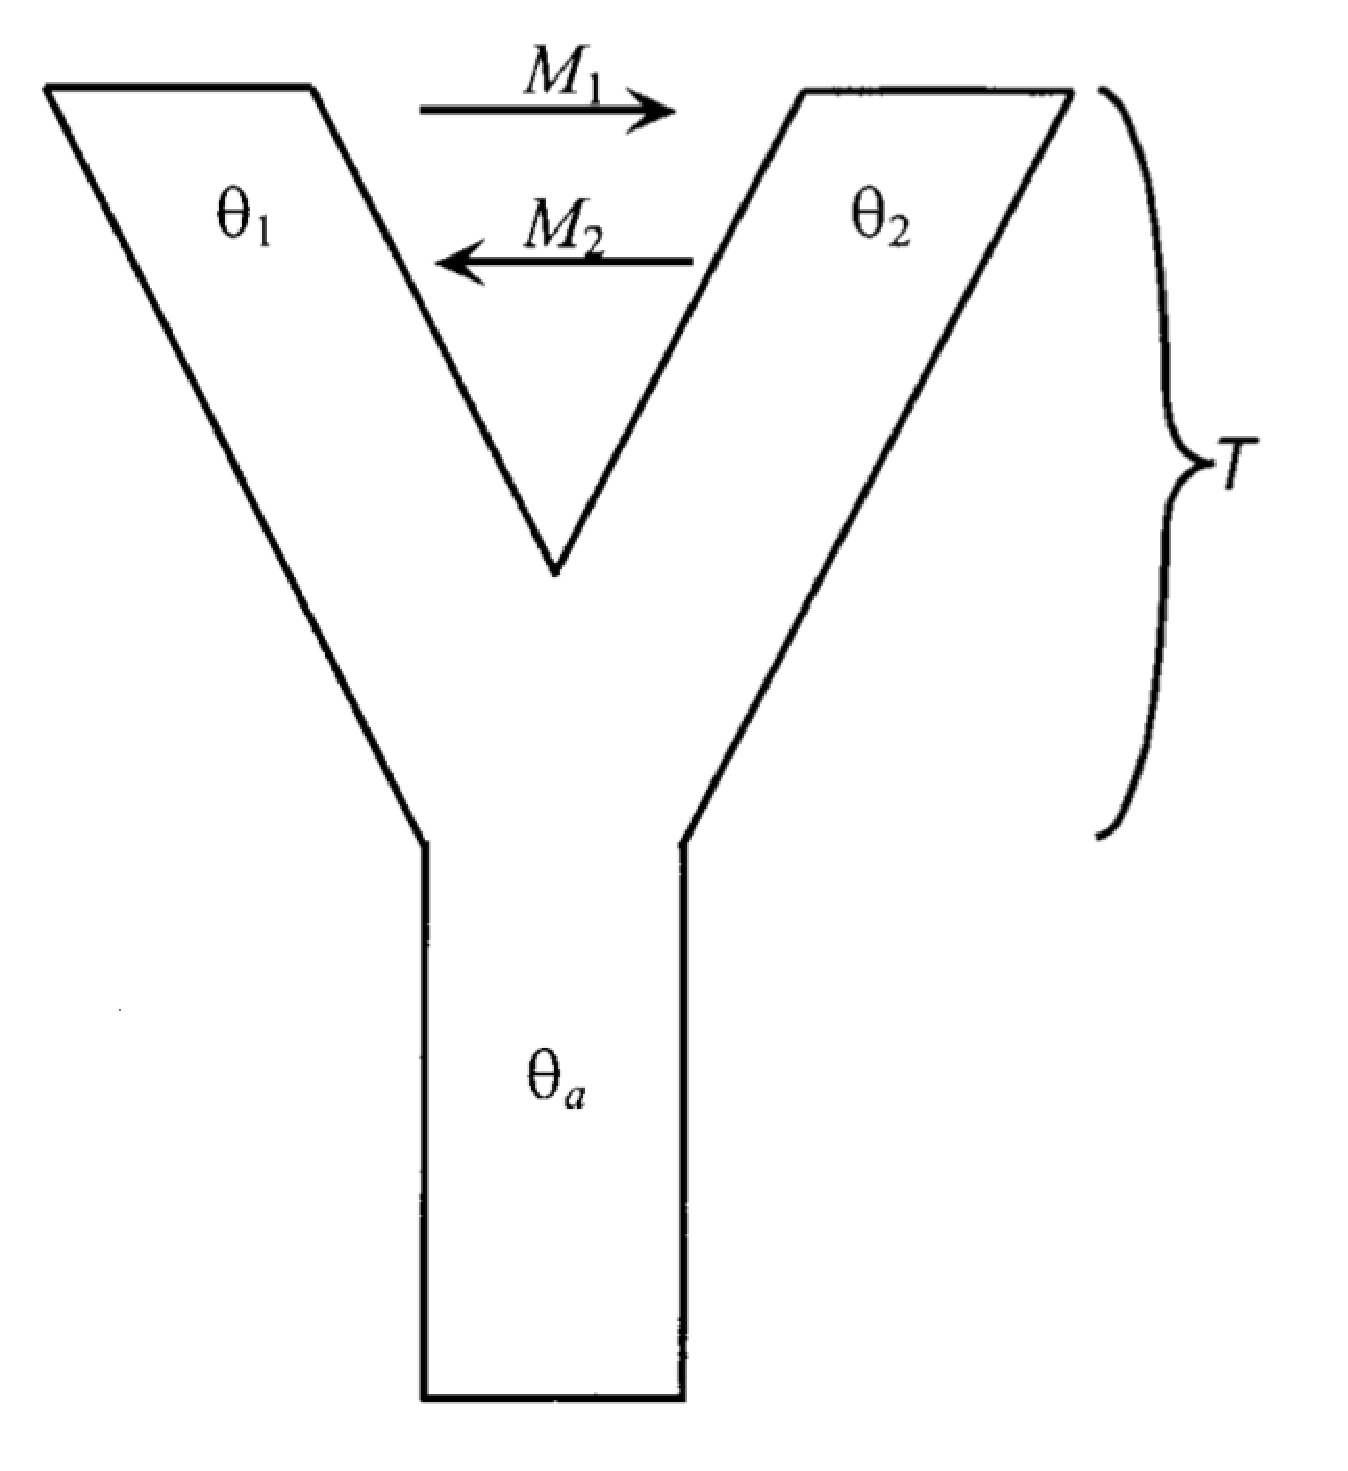
\includegraphics[height=6cm]{nielsen-wakeley.eps}
\end{center}
\caption{The simple model developed by Nielsen and
  Wakeley~\cite{Nielsen-Wakeley-2001}. $\theta_a$ is $4N_e\mu$ in the
  ancestral population; $\theta_1$ and $\theta_2$ are $4N_e\mu$ in the
  descendant populations; $M_1$ and $M_2$ are $2N_em$, where $m$ is
  the backward migration rate; and $T$ is the time since divergence of
  the two populations.}\label{fig:nielsen-wakeley}
\end{figure}

Given that set of parameters, you can probably imagine that you can
calculate the likelihood of the data for a given set of
parameters.\footnote{As with {\tt Migrate}, you can't calculate the
  likelihood explicitly, but you can approximate it
  numerically. See~\cite{Nielsen-Wakeley-2001} for details.} Once you
can do that you can either obtain maximum-likelihood estimates of the
parameters by maximizing the likelihood, or you can place prior
distributions on the parameters and obtain Bayesian estimates from the
posterior distribution. Either way, armed with estimates of
$\theta_a$, $\theta_1$, $\theta_2$, $M_1$, $M_2$, and $T$ you can say
something about: (1) the effective population sizes of the two
populations relative to one another and relative to the ancestral
population, (2) the relative frequency with which migrants enter each
of the two populations from the other, and (3) the time at which the
two populations diverged from one another. Keep in mind, though, that
the estimates of $M_1$ and $M_2$ confound local effective population
sizes with migration rates. So if $M_1 > M_2$, for example, it does
not mean that the fraction of migrants incorporated into population 1
exceeds the fraction incorporated into population 2. It means that the
impact of migration has been felt more strongly in population 1 than
in population 2.

\subsection*{An example}

Orti et al.~\cite{Orti-etal-1994} report the results of phylogenetic
analyses of mtDNA sequences from 25 populations of threespine
stickleback, {\it Gasterosteus aculeatus}, in Europe, North America,
and Japan. The data consist of sequences from a 747bp fragment of
cytochrome $b$. Nielsen and Wakely~\cite{Nielsen-Wakeley-2001} analyze
these data using their approach. Their analyses show that ``[a] model
of moderate migration and very long divergence times is more
compatible with the data than a model of short divergence times and
low migration rates.'' By ``very long divergence times'' they mean $T
> 4.5$, i.e., $t > 4.5N_1$. Focusing on populations in the western
(population 1) and eastern Pacific (population 2), they find that the
maximum likelihood estimate of $M_1$ is 0, indicating that there is
little if any gene flow from the eastern Pacific (population 2) into
the western Pacific (population 1). In contrast, the maximum
likelihood estiamte of $M_2$ is about 0.5, indicating that one
individual is incorporated into the eastern Pacific population from
the western Pacific population every other generation. The
maximum-likelihood estimates of $\theta_1$ and $\theta_2$ indicate
that the effective size of the population eastern Pacific population
is about 3.0 times greater than that of the western Pacific
population.

\subsection*{Extending the approach to multiple populations}

Several years ago, Jody Hey announced the release of {\tt
  IMa2}. Building on work described in Hey and
Nielsen~\cite{Hey-Nielsen-2004,Hey-Nielsen-2007}, {\tt IMa2} allows
you to estimate relative divergence times, relative effective
population sizes, and relative pairwise migration rates for more than
two populations at a time. That flexibility comes at a cost, of
course. In particular, you have to specify the phylogenetic history of
the populations before you begin the analysis.



\section*{Approximate Bayesian computation}

Just when you thought it was safe to go back into the water, I'm going
to complicate things even further.\footnote{Look on the bright
  side. The semester is nearly over. Besides, you need to know a
  little about approximate Bayesian computation in order to write up
  your final problem.} Nielsen, Wakely, and Hey introduced a {\it
  very\/} flexible and {\it very\/} powerful approach for making
inferences about population histories, including the history of
migration among
populations~\cite{Nielsen-Wakeley-2001,Hey-Nielsen-2004,Hey-Nielsen-2007}. It
uses coalescent theory to calculate likelihoods and estimate times of
population divergence, migration rates, and populations sizes in a
surprisingly flexible way, but even it doesn't cover all possible
scenarios. It allows for non-equilibrium scenarios in which the
populations from which we sampled diverged from one another at
different times, but suppose that we think our populations have
dramatically increased in size over time (as in humans) or
dramatically changed their distribution (as with an invasive
species). Is there a way to use genetic data to gain some insight into
those processes? Would I be asking that question if the answer were
``No''?

\section*{An example}

Let's change things up a bit this time and start with an example of a
problem we'd like to solve first. Once you see what the problem is,
then we can talk about how we might go about solving it. The case
we'll discuss is the case of the cane toad, {\it Bufo marinus}, in
Australia.\index{Bufo@\textit{Bufo}!\textit{marinus}}

You may know that the cane toad is native to the American tropics. It
was purposely introduced into Australia in 1935 as a biocontrol agent,
where it has spread across an area of more than 1 million km$^2$. Its
range is still expanding in northern Australia and to a lesser extent
in eastern
Australia~(Figure~\ref{fig:cane-toad-expansion}).\footnote{All of this
  information is from the introduction to~\cite{Estoup-etal-2004}.}
Estoup et al.~\cite{Estoup-etal-2004} collected microsatellite data
from 30 individuals in each of 19 populations along roughly linear
transects in the northern and eastern expansion areas.

\begin{figure}
\begin{center}
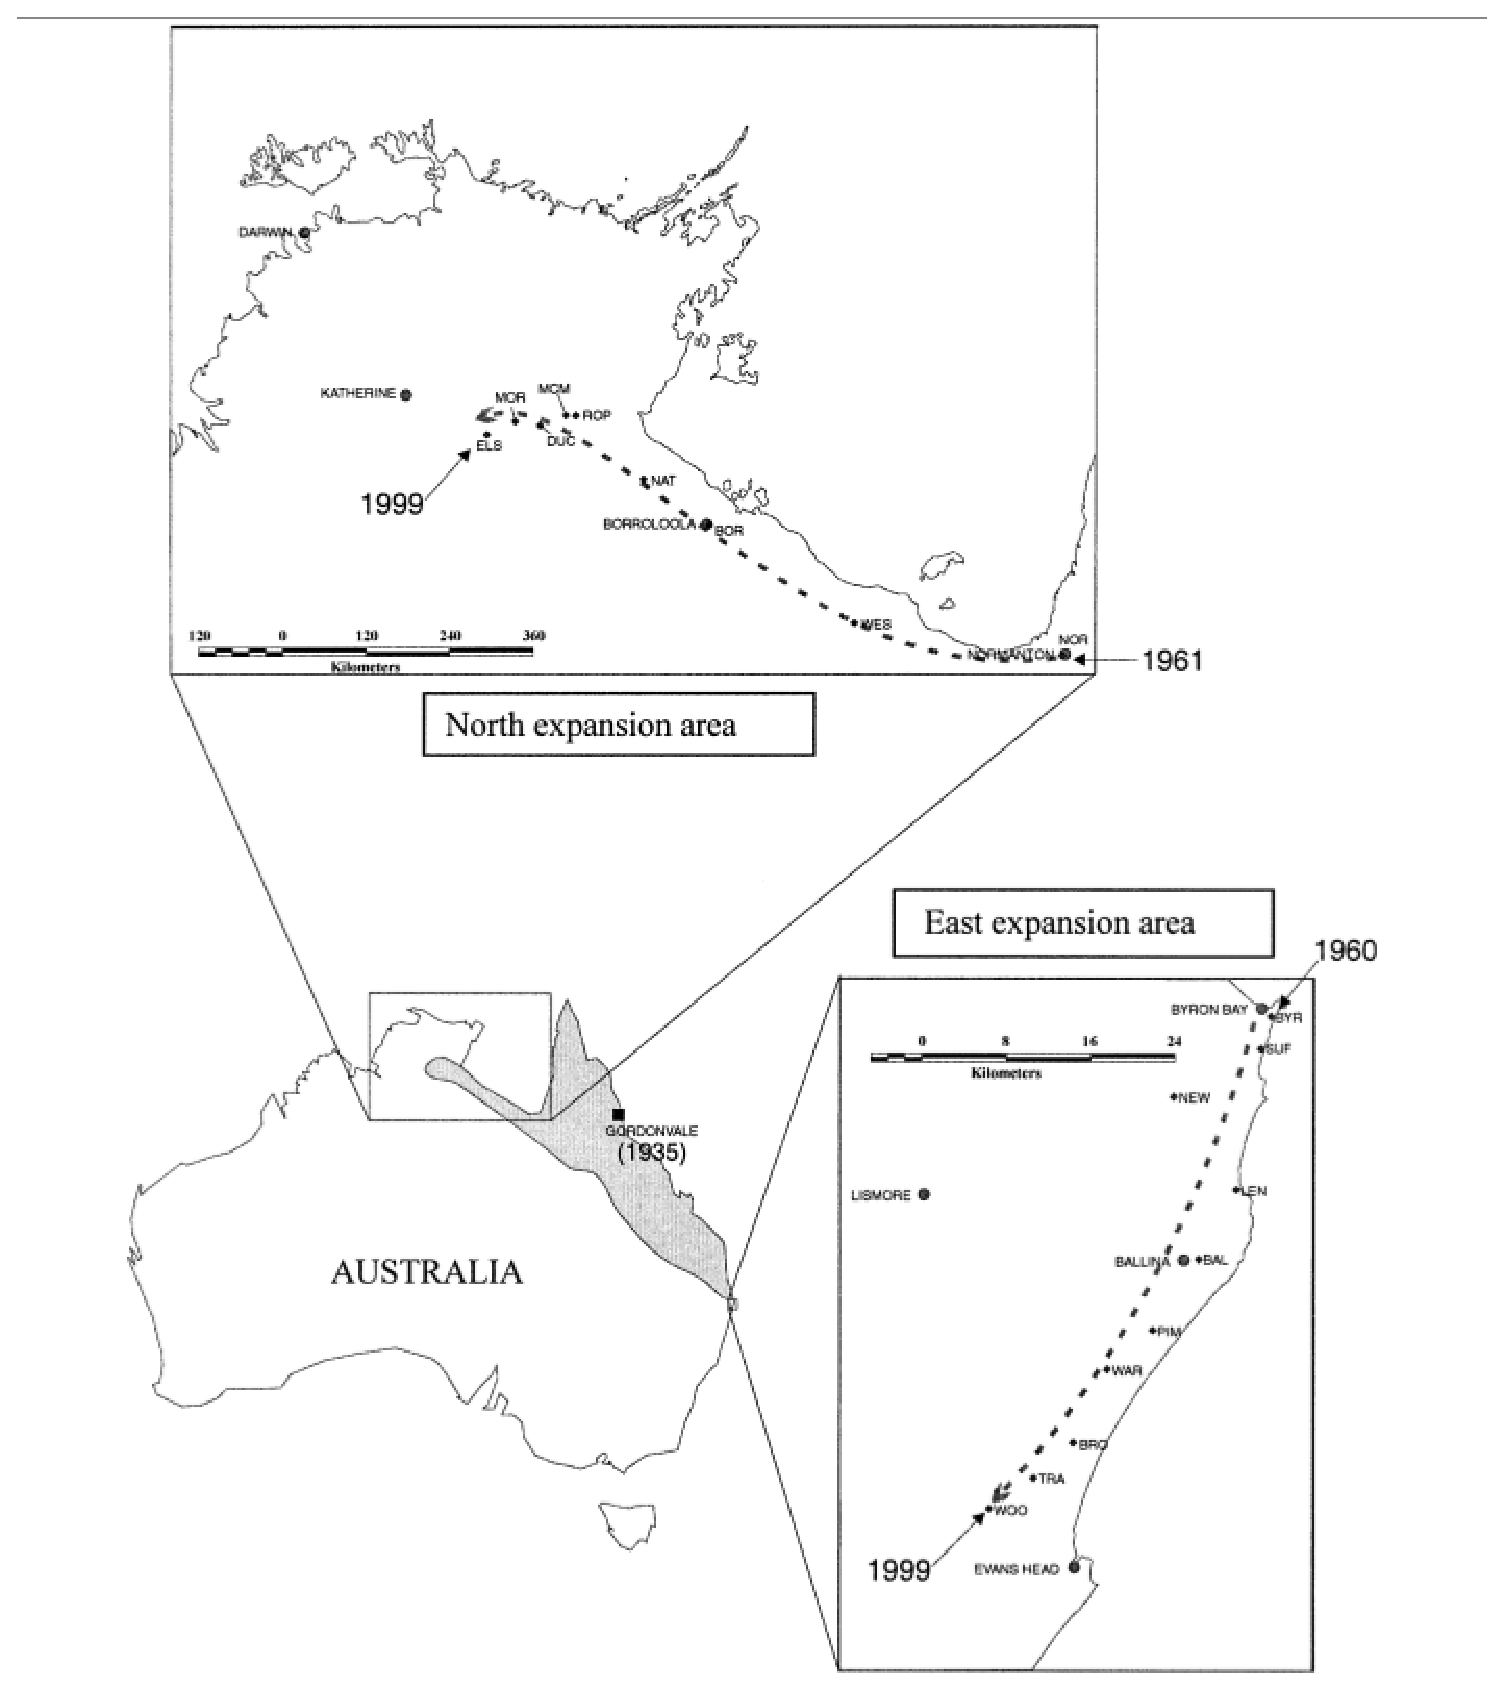
\includegraphics[width=6.0in]{cane-toad-expansion.eps}
\end{center}
\caption{Maps showing the expansion of the cane toad population in
  Australia since its introduction in 1935~(from~\cite{Estoup-etal-2004}).}\label{fig:cane-toad-expansion}
\end{figure}

With these data they wanted to distinguish among five possible
scenarios describing the geographic spread:

\begin{itemize}

\item {\bf Isolation by distance}: As the expansion proceeds, each new
  population is founded by or immigrated into by individuals with a
  probability proportional to the distance from existing populations.

\item {\bf Differential migration and founding}: Identical to the
  preceding model except that the probability of founding a population
  may be different from the probability of immigration into an
  existing population.

\item {\bf ``Island'' migration and founding}: New populations are
  established from existing populations without respect to the
  geographic distances involved, and migration occurs among
  populations without respect to the distances involved.

\item {\bf Stepwise migration and founding with founder events}: Both
  migration and founding of populations occurs only among immediately
  adjacent populations. Moreover, when a new population is
  established, the number of individuals involved may be very small.

\item {\bf Stepwise migration and founding without founder events}:
  Identical to the preceding model except that when a population is
  founded its size is assumed to be equal to the effective population
  size. 

\end{itemize}

That's a pretty complex set of scenarios. Clearly, you could use {\tt
  Migrate} or {\tt IMa2} to estimate parameters from the data Estoup
et al.~\cite{Estoup-etal-2004} report, but would those parameters
allow you to distinguish those scenarios? Not in any straightforward
way that I can see. Neither {\tt Migrate} nor {\tt IMa2} distinguishes
between founding and migration events for example. And with {\tt IMa2}
we'd have to specify the relationships among our sampled populations
before we could make any of the calculations. In this case we want to
test alternative hypotheses of population relationship. So what do we
do?

\section*{Approximate Bayesian Computation}\index{Approximate Bayesian Computation}

Well, in principle we could take an approach similar to what {\tt
  Migrate} and {\tt IMa2} use. Let's start by reviewing what we did
last time\footnote{More accurately, what Peter Beerli, Joe
  Felsenstein, Rasmus Nielsen, John Wakeley, and Jody Hey did} with
{\tt Migrate} and {\tt IMa2}. In both cases, we knew how to simulate
data given a set of mutation rates, migration rates, local effective
population sizes, and times since divergence. Let's call that whole,
long string of parameters $\phi$ and our big, complicated data set
$X$. If we run enough simulations, we can keep track of how many of
those simulations produce data identical to the data we
collected. With those results in hand, we can estimate $P(X|\phi)$,
the likelihood of the data, as the fraction of simulations that
produce data identical to the data we collected.\footnote{The actual
  implementation is a bit more involved than this, but that's the
  basic idea.} In principle, we could take the same approach in this,
much more complicated, situation. But the problem is that there are an
astronomically large number of different possible coalescent histories
and different allelic configurations possible with any one population
history both because the population histories being considered are
pretty complicated and because the coalescent history of every locus
will be somewhat different from the coalescent history at other
loci. As a result, the chances of getting {\it any\/} simulated
samples that match our actual samples is virtually nil, and we can't
estimate $P(X|\phi)$ in the way we have so far.

Approximate Bayesian computation is an approach that allows us to get
around this problem. It was introduced by Beaumont et
al.~\cite{Beaumont-etal-2002} precisely to allow investigators to get
approximate estimates of parameters and data likelihoods in a Bayesian
framework. Again, the details of the implementation get pretty
hairy,\footnote{You're welcome to read the Methods
  in~\cite{Beaumont-etal-2002}, and feel free to ask questions if
  you're interested.} but the basic idea is relatively
straightforward.\footnote{OK. This maybe calling it ``relatively
  straightforward'' is misleading. Even this simplified outline is
  fairly complicated, but compared to some of what you've already
  survived in this course, it may not look too awful.}

\begin{enumerate}

\item Calculate ``appropriate'' summary statistics for your data set,
  e.g., pairwise estimates of $\phi_{ST}$ (possibly one for every
  locus if you're using microsatellite or SNP data), estimates of
  within population diversity, counts of the number of segregating
  sites (for nucleotide sequence data, both within each population and
  across the entire sample). Call that set of summary statistics $S$.

\item Specify a prior distribution for the unknown parameters, $\phi$.

\item Pick a random set of parameter values, $\phi'$ from the prior
  distribution and simulate a data set for that set of parameter
  values.

\item Calculate the same summary statistics for the simulated
  data set as you calculated for your actual data. Call that set of
  statistics $S'$. 

\item Calculate the Euclidean distance between $S$ and $S'$. Call it
  $\delta$. If it's less than some value you've decided on,
  $\delta^*$, keep track of $S'$ and the associated $\phi'$ and
  $\delta$. Otherwise, throw all of them away and forget you ever saw
  them.

\item Return to step 2 and repeat until you you have accepted a large
  number of pairs of $S'$ and $\phi'$.

\end{enumerate}

Now you have a bunch of $S'$s and a bunch of $\phi'$s that produced
them. Let's label them $S_i$ and $\phi_i$, and let's remember what
we're trying to do. We're trying to estimate $\phi$ for our real
data. What we have from our real data is $S$. So far it seems as if
we've worked our computer pretty hard, but we haven't made any
progress. 

Here's where the trick comes in. Suppose we fit a regression to the
data we've simulated
\[
\phi_i = \alpha + S_i\beta + \epsilon \quad ,
\]
where $\alpha$ is an intercept, $\beta$ is a vector of regression
coefficients relating each of the summary statistics to $\phi$, and
$\epsilon$ is an error vector.\footnote{I know what you're thinking to
  yourself now. This doesn't sound very simple. Trust me. It is as
  simple as I can make it. The actual procedure involves local linear
  regression. I'm also not telling you how to go about picking
  $\delta$ or how to pick ``appropriate'' summary statistics. There's
  a fair amount of ``art'' involved in that.} Now we can use that
regression relationship to predict what $\phi$ should be in our real
data, namely
\[
\phi = \alpha + S\beta \quad .
\]
If we throw in some additional bells and whistles, we can approximate
the posterior distribution of our parameters. With that we can get not
only a point estimate for $\phi$, but also credible intervals for all
of its components.\index{Approximate Bayesian Computation!regression}

\section*{Back to the real world\footnote{Or at least something
    resembling the real world}}

OK. So now we know how to do ABC, how do we apply it to the cane toad
data. Well, using the additional bells and whistles I mentioned, we
end up with a whole distribution of $\delta$ for each of the scenarios
we try. The scenario with the smallest $\delta$ provides the best fit
of the model to the data. In this case, that corresponds to model 4,
the stepwise migration with founder model, although it is only
marginally better than model 1 (isolation by distance) and model 2
(isolation by distance with differential migration and founding) in
the northern expansion area~(Figure~\ref{fig:cane-toad-models}).\index{Bufo@\textit{Bufo}!\textit{marinus}}

\begin{figure}
\begin{center}
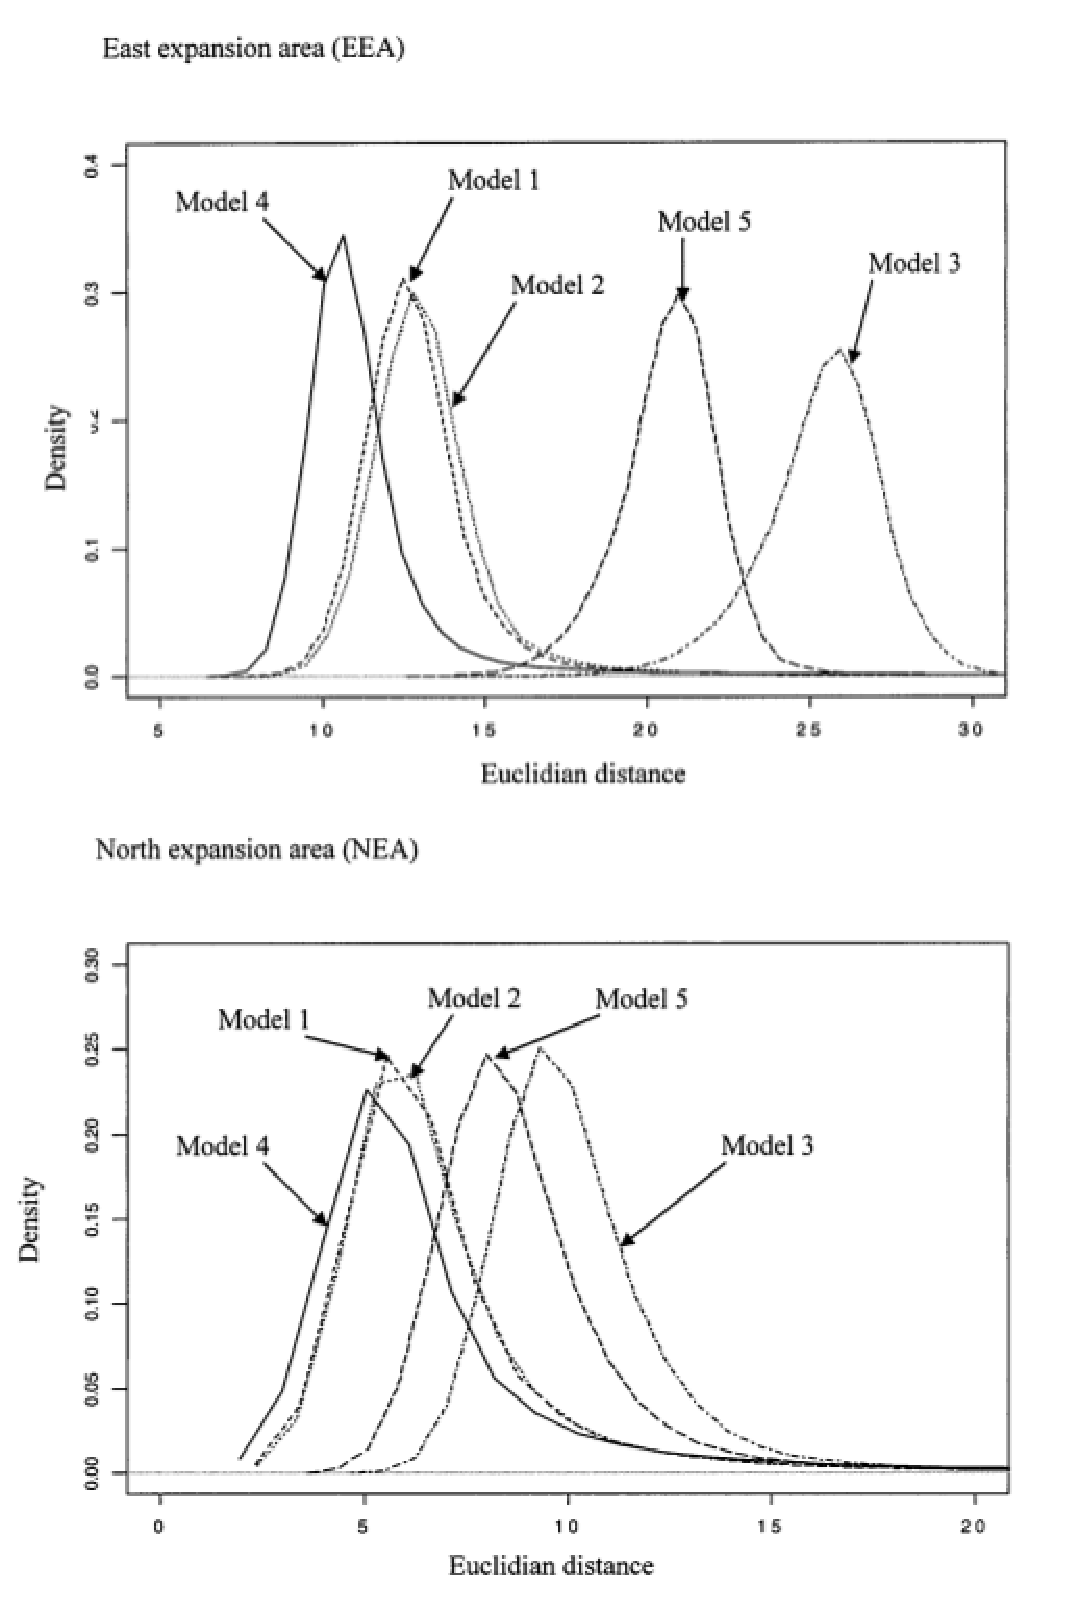
\includegraphics[width=4.5in]{cane-toad-models.eps}
\end{center}
\caption{Posterior distribution of $\delta$ for the five models
  considered in Estoup et al.~\cite{Estoup-etal-2004}.}\label{fig:cane-toad-models}
\end{figure}

Of course, we also have estimates for various parameters associated
with this model: 

\begin{itemize}

\item $N_{e_s}$: the effective population size when the population is
  stable.

\item $N_{e_f}$: the effective population size when a new population
  is founded.

\item $F_R$: the founding ratio, $N_{e_s}/N_{e_f}$.

\item $m$: the migration rate.

\item $N_{e_s}m$: the effective number of migrants per generation.

\end{itemize}

The estimates are summarized in Table~\ref{table:cane-toad}. Although
the credible intervals are fairly broad,\footnote{And notice that
  these are 90\% credible intervals, rather than the conventional 95\%
  credible intervals, which would be even broader.} There are a few
striking features that emerge from this analysis.

\begin{itemize}

\item Populations in the northern expansion area are larger, than
  those in the eastern expansion region. Estoup et
  al.~\cite{Estoup-etal-2004} suggest that this is consistent with
  other evidence suggesting that ecological conditions are more
  homogeneous in space and more favorable to cane toads in the north
  than in the east.

\item A smaller number of individuals is responsible for founding new
  populations in the east than in the north, and the ratio of
  ``equilibrium'' effective size to the size of the founding
  population is bigger in the east than in the north. (The second
  assertion is only weakly supported by the results.)

\item Migration among populations is more limited in the east than in
  the north. 

\end{itemize}

As Estoup et al.~\cite{Estoup-etal-2004} suggest, results like these
could be used to motivate and calibrate models designed to predict the
future course of the invasion, incorporating a balance between gene
flow (which can reduce local adaptation), natural selection, drift,
and colonization of new areas.

\begin{table}
\begin{center}
\begin{tabular}{ccr}
\hline\hline
Parameter & area & mean (5\%, 90\%) \\
\hline
$N_{e_s}$ & east & 744 (205, 1442) \\
         & north & 1685 (526, 2838) \\
$N_{e_f}$ & east & 78 (48, 118) \\
         & north & 311 (182, 448) \\
$F_R$    & east & 10.7 (2.4, 23.8) \\
         & north & 5.9 (1.6, 11.8) \\
$m$      & east & 0.014 ($6.0 \times 10^{-6}$, 0.064) \\
         & north & 0.117 ($1.4 \times 10^{-4}$, 0.664) \\
$N_{e_s}m$ & east & 4.7 (0.005, 19.9) \\
          & north & 188 (0.023, 883) \\
\hline
\end{tabular}
\end{center}
\caption{Posterior means and 90\% credible intervals for parameters of
  model 4 in the eastern and northern expansion areas of {\it Bufo
    marinus}.}\label{table:cane-toad}
\end{table}

\section*{Limitations of ABC}\index{Approximate Bayesian Computation!limitations}

If you've learned anything by now, you should have learned that there
is no perfect method. An obvious disadvantage of ABC relative to
either {\tt Migrate} or {\tt IMa2} is that it is much more
computationally intensive. 

\begin{itemize}

\item Because the scenarios that can be considered are much more
  complex, it simply takes a long time to simulate all of the data. 

\item In the last few years, one of the other disadvantages{\dash}that
  you had to know how to do some moderately complicated scripting to
  piece together several different packages in order to run
  analysis{\dash}has become less of a problem. {\tt popABC}
  (\url{http://code.google.com/p/popabc/} and {\tt DIYABC}
  (\url{http://www1.montpellier.inra.fr/CBGP/diyabc/}) make it {\it
    relatively\/} easy\footnote{Emphasis on ``relatively''.} to
  perform the simulations.

\item Selecting an appropriate set of summary statistics isn't easy,
  and it turns out that which set is most appropriate may depend on
  the value of the parameters that you're trying to estimate and the
  which of the scenarios that you're trying to compare is closest to
  the actual scenario applying to the populations from which you
  collected the data. Of course, if you knew what the parameter values
  were and which scenario was closest to the actual scenario, you
  wouldn't need to do ABC in the first place.

\item In the end, ABC allows you to compare a small number of
  evolutionary scenarios. It can tell you which of the scenarios
  you've imagined provides the best combination of fit to the data and
  parsimonious use of parameters (if you choose model comparison
  statistics that include both components), but it takes additional
  work to determine whether the model is adequate, in the sense that
  it does a good job of explaining the data. Moreover, even if you
  determine that the model is adequate, you can't exclude the
  possibility that there are other scenarios that might be equally
  adequate{\dash}or even better.

\end{itemize}

